\documentclass{beamer}
% \documentclass[handout]{beamer}

    % \usepackage{pgfpages}
    % \pgfpagesuselayout{4 on 1}[a4paper,border shrink=5mm, landscape]


    \usepackage[utf8]{inputenc}
    \usepackage[T1]{fontenc}
    \usepackage[french]{babel}
    \usepackage{url}

    \usetheme{Warsaw}

    \logo{%
            \includegraphics[scale=0.06]{logo}
    }

    % Faire apparaître un sommaire avant chaque section
    \AtBeginSection[]{
        \begin{frame}
            %%% affiche en début de chaque section, les noms de sections et
            %%% noms de sous-sections de la section en cours.
            \tableofcontents[currentsection,hideothersubsections]
        \end{frame} 
    }

    \addtobeamertemplate{footline}{\color{gray}{\insertframenumber{}/\inserttotalframenumber}}

    \title[Projet Auralisation]{Projet Auralisation}
    \institute{L2 SPI TD2\\Novembre 2012 -- Janvier 2013}
    \author{\textsc{Lechat} T. -- \textsc{Wang} X. -- \textsc{Gaborit} M.}
    \date{Christophe Ayrault\\Maître de Conférence\\\bigskip\scalebox{2}{\insertlogo}}

\begin{document}

\begin{frame}
\titlepage
\end{frame}

\begin{frame}
\frametitle{Plan}
\tableofcontents
\end{frame}

\section{Le projet}
\subsection{Contexte}

\begin{frame}

Bref historique :
\begin{itemize}
    \item premières recherches en 1929 par Spandöck
    \item «création» du mot "auralisation" par Kleiner en 1993
\end{itemize}

Aujourd'hui :

\begin{itemize}
    \item application à l'architecture
    \item application à l'acoustique urbaine
    \item application à la réalité virtuelle
    \item travaux sur la psycho-acoustique (sons 3D)
\end{itemize}

\end{frame}

\subsection{Principe de l'auralisation}

\begin{frame}

\begin{figure}
\centering{\includegraphics[width=8.5cm]{principe_1.png}}
\end{figure}

\begin{equation*}
s(t) = e(t)\ast h(t)
\end{equation*}

\end{frame}

\begin{frame}

\begin{figure}
\centering{\includegraphics[width=8.5cm]{principe_2.png}}
\end{figure}

\begin{equation*}
\mathcal{F}\left\{e(t) \ast h(t)\right\} = \hat{E}(F) \cdot \hat{H}(F)
\end{equation*}
\end{frame}


\section{Traitement du signal}

\begin{frame}
\begin{itemize}
    \item normalisation de matrices
    \item détection d'un \textit{bug} dans \textit{Analyseur CTTM}
    \item Réimplémentation de \texttt{fftconv()}
\end{itemize}
\end{frame}

\section{Etude monaurale}

\begin{frame}
\begin{figure}
\centering{\includegraphics[width=8.5cm]{temporel_reverb.png}}
\end{figure}
\begin{center}
Convolution entre une RI de salle réverbérante et un signal ancéhoïque
\end{center}
\end{frame}

\section{Etude binaurale}

\begin{frame}
\begin{figure}
\centering{\includegraphics[width=8.5cm,height=6cm]{rapport_droite.png}}
\end{figure}
\begin{center}
Différences entre les RI droite et gauche en salle réverbérante avec l'oreille droite vers la source
\end{center}
\end{frame}

\begin{frame}
\begin{figure}
\centering{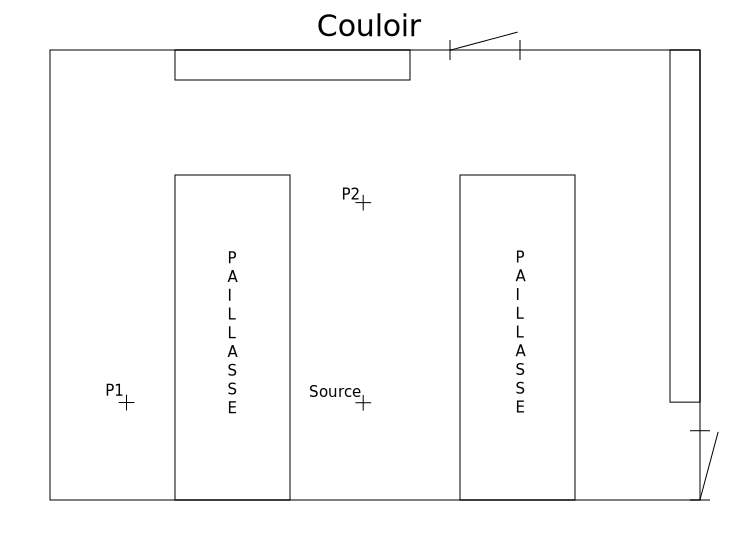
\includegraphics[width=8.5cm]{plan_mersenne.png}}
\end{figure}
\begin{center}
Plan de la salle Mersenne
\end{center}
\end{frame}

\begin{frame}
\begin{itemize}
    \item Écoute par plusieurs personnes : synthèse
    \begin{itemize}
        \item bon repérage dans le plan horizontal
        \item identification du type de salle
    \end{itemize}
    \item Nécessité de prises de RI binaurales
\end{itemize}
 \end{frame}

\section{Conclusion et optimisations possibles}

\begin{frame}

\begin{itemize}
    \item mise en place de l'auralisation assez simple ;
    \item optimisation assez difficiles même si résultats probants ;
    \item prise en compte de la binauralité importante pour l'immersion
\end{itemize}

Optimisations possibles :

\begin{itemize}
    \item prise en compte de la chaine d'excitation et de mesure
    \item amélioration des RI sans changer de source
    \item système CLIO\textsuperscript{\textsc{TM}} (signaux MLS)
\end{itemize}
\end{frame}

\end{document}
